%
%
% UCSD Doctoral Dissertation Template
% -----------------------------------
% https://github.com/ucsd-thesis/ucsd-thesis
%
%
% ----------------------------------------------------------------------
% WARNING: 
%
%   This template has not endorced by OGS or any other official entity.
%   The official formatting guide can be obtained from OGS.
%   It can be found on the web here:
%   http://grad.ucsd.edu/_files/academic-affairs/Dissertations_Theses_Formatting_Manual.pdf
%
%   No guaranty is made that this LaTeX class conforms to the official UCSD guidelines.
%   Make sure that you check the final document against the Formatting Manual.
%  
%   That being said, this class has been routinely used for successful 
%   publication of doctoral theses.  
%
%   The ucsd.cls class files are only valid for doctoral dissertations.
%
%
% ----------------------------------------------------------------------
% GETTING STARTED:
%
%   Lots of information can be found on the project wiki:
%   http://code.google.com/p/ucsd-thesis/wiki/GettingStarted
%
%
%   To make a pdf from this template use the command:
%     pdflatex template
%
%
%   To get started please read the comments in this template file 
%   and make changes as appropriate.
%
%   If you successfully submit a thesis with this package please let us
%   know.
%
%
% ----------------------------------------------------------------------
% KNOWN ISSUES:
%
%   Currently only the 12pt size conforms to the UCSD requirements.
%   The 10pt and 11pt options make the footnote fonts too small.
%
%
% ----------------------------------------------------------------------
% HELP/CONTACT:
%
%   If you need help try the ucsd-thesis google group:
%   http://groups.google.com/group/ucsd-thesis
%
%
% ----------------------------------------------------------------------
% BUGS:
%
%   Please report all bugs at:
%   https://github.com/ucsd-thesis/ucsd-thesis/issues
%
%
% ----------------------------------------------------------------------
% More control of the formatting of your thesis can be achieved through
% modifications of the included LaTeX class files:
%
%   * ucsd.cls    -- Class file
%   * uct10.clo   -- Configuration files for font sizes 10pt, 11pt, 12pt
%     uct11.clo                            
%     uct12.clo
%
% ----------------------------------------------------------------------



% Setup the documentclass 
% default options: 12pt, oneside, final
%
% fonts: 10pt, 11pt, 12pt -- are valid for UCSD dissertations.
% sides: oneside, twoside -- note that two-sided theses are not accepted 
%                            by OGS.
% mode: draft, final      -- draft mode switches to single spacing, 
%                            removes hyperlinks, and places a black box
%                            at every overfull hbox (check these before
%                            submission).
% chapterheads            -- Include this if you want your chapters to read:
%                              Chapter 1
%                              Title of Chapter
%
%                            instead of
%                              1 Title of Chapter
\documentclass[12pt,chapterheads]{ucsd}



% Include all packages you need here.  
% Some standard options are suggested below.
%
% See the project wiki for information on how to use 
% these packages. Other useful packages are also listed there.
%
%   http://code.google.com/p/ucsd-thesis/wiki/GettingStarted



%% AMS PACKAGES - Chances are you will want some or all 
%    of these if writing a dissertation that includes equations.
%  \usepackage{amsmath, amscd, amssymb, amsthm}

%% GRAPHICX - This is the standard package for 
%    including graphics for latex/pdflatex.
\usepackage{scrextend}
\usepackage{pslatex}
\usepackage{graphicx}

%% CAPTION
% This overrides some of the ugliness in ucsd.cls and
% allows the text to be double-spaced while letting figures,
% tables, and footnotes to be single-spaced--all OGS requirements.
% NOTE: Must appear after graphics and ams math
\makeatletter
\gdef\@ptsize{2}% 12pt documents
\let\@currsize\normalsize
\makeatother
\usepackage{setspace}
\doublespace
\usepackage[font=small, width=0.9\textwidth]{caption}

%% SUBFIG - Use this to place multiple images in a
%    single figure.  Subfig will handle placement and
%    proper captioning (e.g. Figure 1.2(a))
% \usepackage{subfig}

%% TIMES FONT - replacements for Computer Modern
%%   This package will replace the default font with a
%%   Times-Roman font with math support.
% \usepackage[T1]{fontenc}
% \usepackage{mathptmx}

%% INDEX
%   Uncomment the following two lines to create an index: 
% \usepackage{makeidx}
% \makeindex
%   You will need to uncomment the \printindex line near the
%   bibliography to display the index.  Use the command
% \index{keyword} 
%   within the text to create an entry in the index for keyword.
%   To compile a LaTeX document with an index the 'makeindex'
%   command will need to be run.  See the wiki for more details.

%% HYPERLINKS
%   To create a PDF with hyperlinks, you need to include the hyperref package.
%   THIS HAS TO BE THE LAST PACKAGE INCLUDED!
%   Note that the options plainpages=false and pdfpagelabels exist
%   to fix indexing associated with having both (ii) and (2) as pages.
%   Also, all links must be black according to OGS.
%   See: http://www.tex.ac.uk/cgi-bin/texfaq2html?label=hyperdupdest
%   Note: This may not work correctly with all DVI viewers (i.e. Yap breaks).
%   NOTE: hyperref will NOT work in draft mode, as noted above.
% \usepackage[colorlinks=true, pdfstartview=FitV, 
%             linkcolor=black, citecolor=black, 
%             urlcolor=black, plainpages=false,
%             pdfpagelabels]{hyperref}
% \hypersetup{ pdfauthor = {Your Name Here}, 
%              pdftitle = {The Title of The Dissertation}, 
%              pdfkeywords = {Keywords for Searching}, 
%              pdfcreator = {pdfLaTeX with hyperref package}, 
%              pdfproducer = {pdfLaTeX} }
% \urlstyle{same}
% \usepackage{bookmark}


%% CITATIONS
% Sets citation format
% and fixes up citations madness
\usepackage{microtype}  % avoids citations that hang into the margin


%% FOOTNOTE-MAGIC
% Enables footnotes in tables, re-referencing the same footnote multiple times.
\usepackage{footnote}
\makesavenoteenv{tabular}
\makesavenoteenv{table}


%% TABLE FORMATTING MADNESS
% Enable all sorts of fun table tricks
\usepackage{rotating}  % Enables the sideways environment (NCPW)
\usepackage{array}  % Enables "m" tabular environment http://ctan.org/pkg/array
\usepackage{booktabs}  % Enables \toprule  http://ctan.org/pkg/array



\begin{document}

%% FRONT MATTER
%
%  All of the front matter.
%  This includes the title, degree, dedication, vita, abstract, etc..
%  Modify the file template_frontmatter.tex to change these pages.
%
%UCSD Master's Thesis - Kevin Chau, Biology 2019
% ----------------------------------------------------------------------
%

\title{Isoform transcriptome of developing brain provides new insights into autism risk variants}

\author{Kevin Khai Chau}
\degreeyear{2019}

\degreetitle{Master of Science}

\field{Biology}

\chair{Lilia M. Iakoucheva}
\cochair{Scott Rifkin}

%  The rest of the committee members  must be alphabetized by last name.
\othermembers{
Barry Grant\\
}
\numberofmembers{3} % |chair| + |cochair| + |othermembers|


%% START THE FRONTMATTER
\begin{frontmatter}

%% TITLE PAGES
\makefrontmatter

%% SETUP THE TABLE OF CONTENTS
\tableofcontents
\listoffigures
\listofsuppfigures
\listoftables

%% ACKNOWLEDGEMENTS
\begin{acknowledgements}
I would like to acknowledge Professor Lilia M. Iakoucheva for her support as the chair of my committee. \par
I would also like to thank my post-doctoral mentor Dr. Pan Zhang for his guidance throughout this project, as well as Dr. Patricia M. Losada, Dr. Akula Bala Pramod, Dr. Jorge Urresti, and Dr. Megha Amar for all of their support. \par
This thesis, in full, is currently being prepared for submission for publication of the material. Chau, Kevin K.; Zhang, Pan; Urresti, Jorge; Amar, Megha; Pramod, Akula Bala; Corominas, Roser; Lin, Guan Ning; Iakoucheva, Lilia M. The thesis author was the primary investigator and author of this material. \par
\end{acknowledgements}


\begin{abstract}
Alternative splicing plays important role in brain development, however its global contribution to human neurodevelopmental diseases (NDD) has not been fully investigated. Here, we examined the relationship between splicing isoform expression and \textit{de novo} loss-of-function mutations implicated in autism. We constructed isoform transcriptome of the developing human brain, and observed better resolution and stronger signals at the isoform-level compared to the gene-level transcriptome. We identified differentially expressed isoforms and isoform co-expression modules enriched in autism loss-of-function mutations. These isoforms have higher prenatal expression, are enriched in microexons, and are co-expressed with a unique set of partners. We experimentally test the impact of splice site mutations in five NDD risk genes, including \textit{SCN2A}, \textit{DYRK1A} and \textit{BTRC}, and demonstrate exon skipping. Furthermore, our results suggest that the splice site mutation in \textit{BTRC} reduces its translational efficiency, likely impacting Wnt signaling through impaired degradation of $\beta$-catenin. We propose that functional effect of mutations associated with human diseases should be investigated at isoform- rather than gene-level resolution.

\end{abstract}


\end{frontmatter}






%% DISSERTATION

% A common strategy here is to include files for each of the chapters. I.e.,
% Place the chapters is separate files: 
%   chapter1.tex, chapter2.tex
% Then use the commands:
%   \include{chapter1}
%   \include{chapter2}
%
% Of course, if you prefer, you can just start with
%   \chapter{My First Chapter Name}
% and start typing away.  
\chapter{Impact of \textit{de novo} Splicing Mutations on Human Brain Spliceoform Dynamics in Autism Spectrum Disorder}
\section{Background}

More than 95\% of multi-exon human genes undergo alternative splicing (AS) and/or use alternative promoters to increase transcriptomic and proteomic diversity  \cite{Pan2008, Wang2008} . As a result, multiple isoforms can be generated from each gene, with an estimated average of five to seven isoforms per gene (Pan et al., 2008; Steijger et al., 2013).  Alternative splicing is highly specific, and expression of isoforms is often restricted to certain organs, tissues or even cell types within the same tissue (Barbosa-Morais et al., 2012; Shalek et al., 2013; Trapnell et al., 2010). In addition, many isoforms are expressed only during specific developmental periods (Kalsotra and Cooper, 2011) . The alternatively spliced isoforms encoded by the same gene can also be expressed at different levels in the same tissue or during the same developmental period \cite{Wang2008} .

The brain is one of the tissues with the highest number of AS events (Calarco et al., 2011; Mele et al., 2015; Raj and Blencowe, 2015; Yeo et al., 2004). Several recent studies demonstrated that processes occurring during neural development, such as cell-fate determination, neuronal migration, axon guidance and synaptogenesis, are controlled by differentially expressed alternatively spliced isoforms (Grabowski, 2011; Kim et al., 2013; Li et al., 2007). Quantitative differences in brain isoform expression have been previously analyzed primarily in the model organisms (Trapnell et al., 2010), and limited to specific brain regions, sets of genes, neuronal cell types or developmental periods (Chen et al., 2008; Shekhar et al., 2016; Zhang et al., 2014). However, the global spatiotemporal diversity of splicing isoform expression within the developing human brain remained relatively unexplored. Furthermore, how disease-associated mutations impact different isoforms is still an open question.

Since many exons are differentially used, it is likely that the disease mutations may selectively impact only isoforms with mutation-carrying exons. In addition, if some isoforms are not expressed at a particular developmental period or in a particular tissue, then the disease mutations affecting such isoforms may not manifest their functional impact at that period or in that tissue. Correlating period- and tissue-specific isoform expression with disease mutations is an important and necessary task for improving our understanding of human diseases.

Investigating the impact of the disease mutations at the isoform-level is also needed, because different protein isoforms have drastically different protein interaction capabilities. We showed that the majority of the isoforms encoded by the same gene share less than a half of their interacting partners in the human interactome network (Yang et al., 2016). This observation points to striking functional differences between splicing isoforms that are not accounted for by the majority of the existing gene-level studies. Our recent work demonstrated that isoform-level networks provide better resolution and depth around disease candidate proteins compared to the gene-level networks (Corominas et al., 2014). 

Integration of brain spatiotemporal transcriptome with the genetic data from exome sequencing studies has provided important insights into neurodevelopmental diseases (NDDs) (Gulsuner et al., 2013; Lin et al., 2015; Parikshak et al., 2013; Willsey et al., 2013). However, most of the recent work in this area was focused on investigation of protein-coding mutations at the gene-level resolution (Chang et al., 2014; Gilman et al., 2012; Gilman et al., 2011; Iossifov et al., 2015; Samocha et al., 2014; Sanders et al., 2015; Uddin et al., 2014). Several studies have explored the role of mutations that dysregulate alternative splicing in relation to other human diseases, and targeted antisense oligonucleotides that correct splicing defects are now being tested in the clinic for myotonic dystrophy, spinal muscular atrophy and Duchenne muscular dystrophy (Bader and Hogue, 2002; Kole et al., 2012). The investigation of splice site-disrupting mutations in relation to NDDs is still lagging behind.

\section{Results}

\subsection{Initial RNA-Seq data processing}

We obtained previously quantified gene-level and transcript-level RNA-Seq data from the BrainSpan Atlas of the Developing Human Brain, which includes data from multiple regions of post-mortem brain tissue from clinically unremarkable donors aged between 8 weeks post-conception to 40 years of age [CITATION]. We then filtered this dataset for those features that are expressed in the brain and performed sample connectivity calculations to identify sample outliers (\textbf{Materials and Methods}). As a result, we obtained spatiotemporal expression profiles for 100,754 unique brain-expressed isoforms corresponding to 26,307 genes ($\sim$ 3.83 isoforms/gene). \par

In order to model latent batch effects, we performed surrogate variable analysis, taking into account sample age, region, ethnicity, study site, and sex as covariates [CITATION]. We chose to use 16 surrogate variables in our downstream analyses based on the collective evidence from principal components analysis, relative log expression, and the distribution of null nominal p-values from our differential expression analyses (\textbf{Materials and Methods}, \textbf{Supplementary Figure 2}). 

\subsection{Modeling the timeline of expression across neurodevelopment}

We performed differential expression analysis between all adjacent developmental periods as well as between all prenatal and postnatal samples using the \textit{limma} R package ([CITATION], \textbf{Materials and Methods}). We find a total of 16.88\% of brain-expressed isoforms as differentially expressed between any two adjacent developmental periods, with a majority of those DE isoforms contributed by P06P07 (6.86\%) and P07P08 (6.83\%), indicating high levels of expression regulation from late-fetal to neonatal ages (FDR-adjusted P-value $\leq$ 0.05, abs(FoldChange) $\geq$ 1.5). Among just prenatal contrasts, we find 9.83\% of brain-expressed isoforms to be DE (P02P03, 1.44\%; P03P04, 0.76\%; P04P05, 1.61\%; P05P06, 0.75\%; P06P07, 6.86\%); among postnatal contrasts, 5.06\% (P08P09, 2.13\%; P09P10, 1.76\%; P10P11, 1.24\%; P11P12, 0.67\%; P12P13, 0.51\%). 

\subsection{Functional impact of \textit{de novo} splice site mutations in temporally regulated isoforms}

We explored the functional impact of \textit{de novo} mutations affecting splice sites of four genes that are implicated in autism spectrum disorder or schizophrenia that transcript differentially expressed transcripts (SCN2A, DYRK1A, DLG2, and CELF2) using exon trapping assays (\textbf{Experimental Procedures}). The de novo splice site mutation in SCN2A (chr2:166187838, A:G, acceptor site) from a schizophrenia patient (Fromer et al., 2014) caused out-of-frame exon skipping and potentially inclusion of 30 new amino acids into the translated protein and ending with a premature stop codon (Figure 4a). In contrast, the de novo splice site mutation in DYRK1A (chr21: 38865466, G:A, donor site), identified through exome sequencing of autism patients (O'Roak et al., 2012b), caused an in-frame exon skipping, potentially producing a different variant of the same protein (Figure 4b). In case of DLG2 (chr11: 83194295, G:A, donor site), the de novo mutation from a schizophrenia patient (Fromer et al., 2014) affects a splice site adjacent to the exon five, which is alternatively spliced in the WT isoforms (Figure 4c). We constructed a minigene that includes exon five together with the preceding exon four, and observed that exon five is constitutively spliced out from our construct independently on the presence of mutation. However, the mutation caused partial (i.e. 65bp) intron inclusion downstream from exon four. At the translational level, this mutation would likely result in the protein that is truncated one residue after the end of exon 4 due to a premature stop codon. Finally, CELF2 mutation (chr10: 11356223, T:C, donor site) identified in a patient with schizophrenia (Xu et al., 2011) affects an alternatively used splice site, which also maps to an exonic region of another alternatively spliced isoform. When cloned into the exon trapping vector, the transcript generated from the WT minigene included the isoform carrying longer exon with mutation (Figure 4d). Thus, after introducing the mutation, no difference between WT and mutant constructs was observed. This is not surprising given the fact that the splice site mutation behaves like exonic missense mutation in the isoform predominantly expressed from our construct. These results suggest that mutations could impact different isoforms of the same gene by different mechanisms, i.e. splice site mutation in one isoform could represent a missense mutation in another isoform. In summary, the above observations showcase different scenarios of the impact of splice site mutations on genes and confirms the need to investigate functional impact of mutations at the isoform- rather than the gene-level resolution.\par

We mapped these mutations to our temporally differentially expressed isoforms 

\subsection{Weighted co-expression network analysis}

We applied the \textit{WGCNA} R package to the transformed counts matrix to construct three different isoform co-expression networks: one with all samples, one with just prenatal samples, and one with just postnatal samples. Interestingly, we identify far more modules in the postnatal-specific co-expression network (79 modules) than the full network (62 modules) and the prenatal network (35 modules).

\section{Materials and Methods}
All analyses were performed using R version $\geq$ 3.5.1. False discovery rate (FDR) adjustment was used to correct for multiple hypothesis testing with a significance threshold of 0.05.

\subsection{Pre-processing of RNA-Seq data}
We downloaded RNA-Seq quantification data from the BrainSpan Atlas of the Developing Human Brian [CITATION]. This resource consists of both gene-level and isoform-level RNA-Seq derived from post-mortem brain tissue from 57 donors aged between 8 weeks post-conception through 40 years, across a number of different brain regions, for a total of 606 initial samples. This data was aligned using STAR and quantified with RSEM with the Gencode V19 human reference genome, resulting in counts and TPM matrices for both datasets [REFERENCE]. These matrices were filtered by applying a filter of TPM $\geq$ 0.1 in at least 25\% of samples in both data sets; we further restricted the data to only include genes with at least one retained isoform per the isoform-level filter and vice-versa, resulting in a total of 100,734 retained isoforms.\par

Sample connectivity analysis was performed in order to detect outliers as previously described [CITATION]. In summary, biweight midcorrelation was calculated among sample expression vectors in both the expression-filtered gene-level and expression-filtered isoform-level datasets. These values were converted into Z-scores. 55 samples were identified as having sample connectivity Z-scores $\leq$ -2 and were removed from downstream analysis.

\subsection{Validation of isoform expression with qPCR}
We used qPCR to estimate the relative isoform expression of 14 genes from independent brain samples, and compared it to the computationally assigned values. We used RNA from a frontal lobe tissue sample of a 22 weeks old female (fetal brain), and RNA from cerebral cortex tissue sample of a 27 years old female (adult brain) (AMSBIO, UK), corresponding to P06 (late mid-fetal) and P12 (young adult) in the BrainSpan data. The BrainSpan isoform expression data was then compared to the qPCR experimental expression results as described below. \par

We first selected multi-isoform genes carrying at least two isoforms that are expressed during P6 and P9 periods. To select the genes, we used the following criteria: (1) computationally assigned expression difference between two isoforms has to be at least 2-fold; (2) to ensure that isoforms are expressed within the detection limits, the expression of one isoform has to be $\geq$40 TPM, while the expression of the other isoform has to be $\geq$10 TPM. We randomly selected 14 genes from the ones that passed these criteria to test by qPCR from independent samples. Primers were designed using exon-exon junctions specific for each of the selected isoforms. We reverse transcribed 3 $\mu$g of RNA using SuperScript II Kit (Invitrogen) to cDNA, following manufacturer’s instructions. Then, the cDNA was diluted ten times to use it as a template for the qPCR reaction. SYBR Green II Master Mix (Invitrogen) was used for the qPCR reaction, performed in a CFX Connect 96X Thermal Cycler, using standard parameters for SYBR Green. Relative expression between each isoform in the two samples was calculated by normalizing each expression value against two housekeeping genes (RPL28 and MRSP36) as control using QIAGEN control primers, and $\Delta\Delta$t method was applied using the CFX Manager Software.

\subsection{Normalization and differential expression analysis}
To normalize the isoform counts data for between-sample comparability, we first performed surrogate variable analysis to detect latent batch effects [CITATION], relying on evidence from a combination of principal components analysis, relative log expression and p-value distribution visualizations to determine the number of surrogate variables that minimizes latent batch effects while avoiding the problem of overfitting (Supplemental Figure 1). Here, we proposed to use 16 surrogate variables for downstream analysis\par

Differential expression analysis of normalized isoform counts data was performed using the \textit{limma} R package. At its core, \textit{limma} performs differential expression analysis by fitting a linear model to each isoform expression vector. However, since simply fitting a linear model generally produces low-powered results, \textit{limma} leverages the highly-parallel nature of genomic data to borrow and incorporate strength from every isoform linear model. Further, it is highly flexible and able to model for many contrasts at once as one whole integrated experiment. These linear models are then processed using parametric empirical Bayes, which, given the parallel nature of these isoform models, incorporates global and local expression variabilities, thereby increasing the overall degrees of freedom for the estimation of isoform-wise variance. Further, \textit{limma} is also able to account for nested experiment designs, similar to fitting a linear mixed effects model, through the \textit{duplicateCorrelation} function. The BrainSpan data is designed with multiple region measurements per individual, such that there are multiple expression measurements per individual "block." The \textit{duplicateCorrelation} function of \textit{limma} is used to calculate the consensus correlation, with the constraint that all isoforms share the same intrablock consensus correlation, which is then incorporated into the linear model to account for this nested data structure. 

\subsection{Minigenes cloning}
We selected five switch genes (SNC2A, DYRK1A, CELF2, DLG2 and BTRC) for the experiments. We cloned the exons of these genes that are likely impacted by splice site mutations, together with the ~1kb of their flanking intronic sequence. The constructs were cloned into pDESTSplice exon trapping expression vector (Kishore et al., 2008). The site-directed mutagenesis by two-step stich PCR was performed to introduce the mutation affecting the splice site.\par

The minigenes were generated by PCR-amplifying the desired sequences from genomic DNA (Clontech). Primers were designed for each minigene, and attB sites were added at the 5’ end of the primers. The sequences of the primers were as follows: (1) SCN2A; Fw: GGAAGCTATGTTTAGCCAGGATACATTTGG, Rv: CCAGATGATGTCCCCTCCCTACATAGTCC;(2) DYRK1A: Fw: GTTGGGAAAATTTCCCCCTATTTAAGC, Rv: CCCAGAGGCTTAATAAAGTATGGACC; (3) CELF2: Fw: GGAGTTGGAATGACAGACGTTCACATGC, Rv: CCGCTGTGGGCTGAGGATCAGTTTCC; (4) DLG2: Fw: GAGGTTCAGAGACATTCAATTCCC, Rv: CTTGATGCTGTCCAGATAATGC; (5) BTRC: Fw: GGGCCTCAGAATGACACAGTACG, Rv: GAACTTGCGTTTCTTGTTTTTGCC. After PCR amplification, amplicons were loaded in a 1\% low EEO agarose gel (G-BioSciences) and purified using the QIAquick Gel Extraction Kit (QIAGEN) following manufacturer’s instructions. Purified amplicons were subcloned into pDON223.1 expression vector using the BP-Gateway System (Invitrogen). At least six different clones for each minigene were sequenced to verify correct sequences of the minigenes. The clone with the desired sequence and highest DNA concentration was used for subcloning into the pDESTSplice expression vector (Addgene) using the LR-Gateway System (Invitrogen).

\subsection{Weighted co-expression network analysis}
Co-expression networks were constructed using the \textit{WGCNA} R package. This network construction package operates under the scale-free topology criterion, such that the given network has a degree distribution which follows a power law, and calculates pairwise correlations among the isoform expression data. We first transformed the counts data by adjusting the counts values using information from the surrogate variable analysis and incorporating any relevant covariates [CITE LINEAR MODELS]. This transformed counts matrix was then tested for scale-free topology, and the network was constructed blockwise using three blocks and the power estimate result from the scale-free topology correlation calculations. Three networks were created: one using all available samples, one using just prenatal samples, and one using just postnatal samples

\subsection{\textit{de novo} splice site mutations}
Variant calling was performedd on \textit{de novo} mutations from [	HOW??] from both case and control autism cohorts from the Simons Simplex Consortium (SSC) and REACH [EXPAND ACRONYM]. These datasets include [N] families with autistic children.

\section{Discussion}

\chapter{Single-Cell RNA-Seq of Mouse Models}
something
\section{16p11.2}
\section{Cul3 Knockout Mice}
\chapter{Just a Test}
This is only a test.
\section{A section}
Lorem ipsum dolor sit amet, consectetuer adipiscing elit. Nulla odio
sem, bibendum ut, aliquam ac, facilisis id, tellus. Nam posuere pede
sit amet ipsum. Etiam dolor. In sodales eros quis pede.  Quisque sed
nulla et ligula vulputate lacinia. In venenatis, ligula id semper
feugiat, ligula odio adipiscing libero, eget mollis nunc erat id orci.
Nullam ante dolor, rutrum eget, vestibulum euismod, pulvinar at, nibh.
In sapien. Quisque ut arcu. Suspendisse potenti. Cras consequat cursus
nulla.

\subsection{A Figure Example}
\label{ssec:figure_example}

This subsection shows a sample figure.

\begin{figure}[h] 
  \centering
  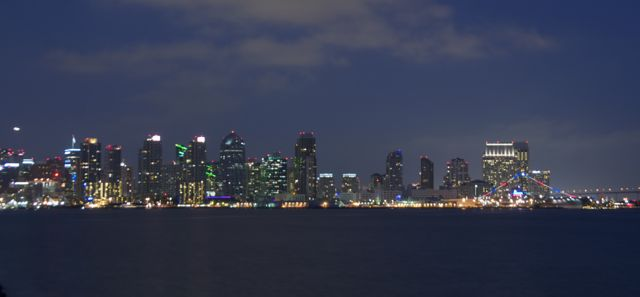
\includegraphics[width=0.5\textwidth]{sandiego}
  \caption[A picture of San Diego. Short figure caption must be \protect{$< 4$} lines in the list of figures]
{A picture of San Diego.  Short figure caption must be \protect{$< 4$} lines in the list of figures and match the start of the main figure caption verbatim. Note that figures must be on their own line (no neighboring text) and captions must be single-spaced and appear \protect\textit{below} the figure.  Captions can be as long as you want, but if they are longer than 4 lines in the list of figures, you must provide a short figure caption.\index{SanDiego}}
  \label{fig:sandiego}
\end{figure}

\subsection{A Table Example}

While in Section \ref{ssec:figure_example} Figure \ref{fig:sandiego} we had a majestic figure, here we provide a crazy table example.


%%%% TABLE 1 %%%%
\vspace{0.25in}
\begin{table}[!ht]
\caption[A table of when I get hungry.  Short table caption must be \protect{$< 4$} lines in the list of tables]{A table of when I get hungry. Short table caption must be \protect{$< 4$} lines in the list of tables and match the start of the main table caption verbatim.  Note that tables must be on their own line (no neighboring text) and captions must be single-spaced and appear \protect\textit{above} the table.  Captions can be as long as you want, but if they are longer than 4 lines in the list of figures, you must provide a short figure caption.}

\vspace{-0.25in}
\begin{center}
\begin{tabular}{|p{1in}|p{2in}|p{3in}|}

\hline
Time of day & Hunger Level & Preferred Food \\

\hline
8am & high & IHOP (French Toast) \\

\hline
noon & medium & Croutons (Tomato Basil Soup \& Granny Smith Chicken Salad) \\

\hline
5pm & high & Bombay Coast (Saag Paneer) or Hi Thai (Pad See Ew) \\

\hline
8pm & medium & Yogurt World (froyo!) \\

\hline
\end{tabular}
\end{center}
\label{tab:analysis3}
\end{table}



%% APPENDIX
\appendix
\chapter{Final notes}
%%What to do about things \cite{Martin_1983}.  What did he say \cite{Rilling_Insel_1999}.
  Remove me in case of abdominal pain.



%% END MATTER
% \printindex %% Uncomment to display the index
% \nocite{}  %% Put any references that you want to include in the bib 
%               but haven't cited in the braces.
\bibliographystyle{unsrt}  %% This is just my personal favorite style. 
%                              There are many others.
%\setlength{\bibleftmargin}{0.25in}  % indent each item
%\setlength{\bibindent}{-\bibleftmargin}  % unindent the first line
%\def\baselinestretch{1.0}  % force single spacing
%\setlength{\bibitemsep}{0.16in}  % add extra space between items
\bibliography{references/test_ref}  %% This looks for the bibliography in template.bib 
%                          which should be formatted as a bibtex file.
%                          and needs to be separately compiled into a bbl file.
\end{document}

